\documentclass[11pt,a4paper]{article}
\usepackage[hangul]{kotex}
\usepackage{amsmath,amssymb}
\usepackage{graphicx}
\usepackage{booktabs}
\usepackage{hyperref}
\usepackage[margin=2.5cm]{geometry}
\usepackage{natbib}
\usepackage{float}
\usepackage{multirow}
\usepackage{array}
\usepackage{caption}
\usepackage{subcaption}
\usepackage{xcolor}
\usepackage{enumitem}
\setlength{\parskip}{0.5em}

\title{\textbf{Gaia: 토양 미생물 군집 이해와 농업 예측을 위한\\토양 특화 기반 모델}}

\author{
  남하진 (Hajin Nam) \\
  자연과학대학 수학과 \\
  계명대학교, 대구, 대한민국 \\
  \texttt{hajin0127@gmail.com} \\
  코드: \url{https://github.com/Kimchikilla/Gaia}
}

\date{2026년 4월}

\begin{document}
\maketitle

\begin{abstract}
토양 미생물 군집은 토양 건강, 농업 생산성, 그리고 지구 생물지구화학적 순환에 영향을 미치는 복잡한 생태 시스템이다. MGM(Microbiome General Model)과 같은 최근의 기반 모델은 미생물 군집 시퀀스에 대한 자기지도학습 사전학습의 가치를 보였지만, 토양 미생물의 고유한 특성에 특화된 모델은 아직 없었다. 본 논문에서는 \textbf{Gaia}를 제안한다. Gaia는 MGnify(2,790), Earth Microbiome Project(4,628), Naylor 외 가뭄 스트레스 실험(623), BonaRes Westerfeld 20년 장기 시험(288) 등 4개 공개 데이터베이스에서 수집한 8,329개 토양 샘플로 MGM을 추가 사전학습한 토양 특화 기반 모델이다. 우리는 사전학습된 지식을 보존하면서 토양 특이 분류군을 통합하는 2단계 학습 전략을 통해 미생물 어휘를 9,669개에서 12,916개 속(genus)으로 확장했다. Gaia는 생물군계 분류, 가뭄 검출, 풍부도 재구성, 농업 관리 분류, 토양 화학 예측, 수확량 예측(현재/미래), 탄소 추정, 기능 프로파일 분석 등 10가지 벤치마크 작업에서 평가되었다. Gaia는 생물군계 분류(98.6\% vs 98.7\%)와 가뭄 검출(91.9\% vs 92.0\%)에서 Random Forest와 거의 동등한 성능을 보였고, 시간적 수확량 예측($R^2$=0.541 vs 0.504)에서는 우월한 성능을 보였다. 추가로 Gaia는 미생물 조성만으로 토양 pH($R^2$=0.947), 총 탄소($R^2$=0.829), 현재 수확량($R^2$=0.873)을 예측한다. 기능 프로파일 분석은 가뭄 조건이 탄소 분해 활성을 98.6\% 증가시키고 질소 고정을 13.4\% 감소시킨다는 것을 보여, 토양 기능 저하의 미생물 메커니즘을 제시한다. 분포 외(out-of-distribution) 일반화를 검증하기 위해 학습에 사용되지 않은 Bernburg 장기 시험(96 샘플)으로 평가한 결과, 선형 프로빙(linear probing)에서 Gaia는 6개 작업 중 5개에서 RF를 능가했고(총 탄소 $R^2$=0.718 vs 0.357), 진정한 zero-shot 사이트 간 전이(Westerfeld로 학습 후 Bernburg 시험)에서는 3개 회귀 작업 모두에서 RF를 능가했다. 특히 pH에서는 RF가 완전히 실패($R^2$=$-$0.515)한 반면 Gaia는 $R^2$=0.393을 달성했다. 모든 작업에서 학습 데이터 양에 따라 성능이 일관되게 향상되어, 본 결과가 잠재력을 과소평가하고 있음을 시사한다. Gaia의 고유한 강점인 풍부도 재구성, 합성 군집 생성, 시간 예측은 단순 특징 기반 방법으로는 불가능한 작업을 가능케 함으로써 전통적 머신러닝을 보완한다. 모든 코드, 데이터 파이프라인, 모델 가중치, 벤치마크 스크립트는 Apache 2.0 라이선스로 \url{https://github.com/Kimchikilla/Gaia}에 공개되어 있다.
\end{abstract}

\textbf{핵심어:} 토양 미생물 군집, 기반 모델, 트랜스포머, GPT-2, 전이 학습, 정밀 농업, 탄소 격리, 가뭄 검출

\section{서론}

\subsection{토양 미생물 군집의 중요성}

토양은 지구상에서 생물다양성이 가장 높은 서식지이다. 토양 1그램에는 약 $10^9$개의 미생물 세포가 있으며, 수천 종의 분류군이 복잡한 생태적 상호작용을 한다. 이러한 미생물 군집은 영양분 순환, 유기물 분해, 식물 생장 촉진, 병원균 억제, 탄소 격리 등 핵심 과정을 매개한다. 토양 미생물 군집의 조성과 기능은 농업 생산성, 생태계 회복력, 그리고 기후 변화와 관련된 지구 생물지구화학적 순환에 직접적인 영향을 미친다.

고처리량 시퀀싱 기술이 토양 미생물 군집을 종합적으로 특성화할 수 있게 되었음에도, 미생물 군집 데이터를 실용적 통찰로 전환하는 것은 여전히 어려운 과제이다. 토양 미생물 군집은 보통 16S rRNA 앰플리콘 시퀀싱이나 샷건 메타게놈 분석으로 특성화되며, 샘플당 100--500개 이상의 분류군에 걸친 속 수준의 풍부도 프로파일을 생성한다. 이러한 데이터의 높은 차원성, 희소성, 생태적 복잡성은 분석에 큰 도전이 된다.

\subsection{전통적 접근법의 한계}

기존 토양 미생물 분석은 주로 Random Forest \citep{breiman2001random} 같은 전통적 머신러닝에 의존해 왔다. 고차원 희소 데이터에 강건하고 특성 중요도를 통한 해석이 쉽기 때문이다. 그러나 이러한 방법은 다음과 같은 근본적 한계가 있다:

\begin{itemize}[leftmargin=1.5em]
    \item \textbf{독립성 가정}: 각 분류군을 독립 특성으로 처리하여 공출현 패턴, 대사 의존성, 경쟁적 상호작용 같은 생태적 관계를 무시한다.
    \item \textbf{작업별 학습}: 예측 작업마다 별도의 모델을 학습해야 하며, 응용마다 라벨 데이터가 필요하다.
    \item \textbf{생성 능력 부재}: 새로운 미생물 프로파일을 생성하거나, 누락된 분류군을 예측하거나, 가상의 군집 상태를 합성할 수 없다.
    \item \textbf{시간적 이해 제한}: 현재 미생물 조성으로 미래 토양 상태를 예측하려면 군집 동역학에 대한 이해가 필요한데, 특성 기반 방법은 이를 포착할 수 없다.
\end{itemize}

\subsection{기반 모델 접근법}

자기지도학습으로 대규모 비라벨 코퍼스에 사전학습된 기반 모델은 자연어 처리 \citep{brown2020language}, 컴퓨터 비전 \citep{dosovitskiy2020image}, 단백질 구조 예측 \citep{jumper2021highly}을 변혁시켰다. 이 모델들은 범용 표현을 학습하여 미세 조정(fine-tuning)을 통해 다운스트림 작업에 효율적으로 적응할 수 있고, 제한된 작업별 데이터로도 최첨단 성능을 달성한다.

최근 이 접근법은 미생물 군집 분석으로 확장되었다. MGM(Microbiome General Model) \citep{mgm2024}은 트랜스포머 기반 언어 모델이 풍부도 순서로 정렬한 속 시퀀스를 미생물 ``언어''의 ``문장''으로 처리함으로써 미생물 군집의 의미있는 표현을 학습할 수 있음을 보였다. MGM은 모든 생물군계(장, 해양, 담수, 토양 등)에 걸친 263,302개 MGnify 샘플로 사전학습되었으며 다양한 분류 작업에서 강한 성능을 보인다.

동시에 BiomeGPT는 비슷한 접근법을 인간 장 미생물 군집에 특화하여 염증성 장 질환 분류에서 뛰어난 성능(AUROC 0.999)을 달성했다. 이러한 성공은 도메인 특화 기반 모델이 범용 모델보다 특수 작업에서 더 나은 성능을 낼 수 있음을 시사한다.

\subsection{공백: 토양 특화 기반 모델}

그러나 토양 미생물 군집을 위해 특별히 개발된 기반 모델은 아직 없다. 다른 환경과 구별되는 토양의 고유한 특성에도 불구하고 말이다:

\begin{itemize}[leftmargin=1.5em]
    \item \textbf{예외적인 다양성}: 토양 샘플은 보통 100--500개 이상의 속을 포함하며, 인체 관련 환경보다 훨씬 많다.
    \item \textbf{강한 환경 구배}: 토양 pH, 수분, 유기물, 온도가 뚜렷한 생태적 적소를 만든다.
    \item \textbf{느린 시간 동역학}: 빠르게 변하는 인간 장 미생물과 달리 토양 군집은 수개월에서 수년에 걸쳐 변화한다.
    \item \textbf{농업 관리의 영향}: 경운, 시비, 관개, 작물 윤작이 토양 미생물 구조를 깊이 형성한다.
    \item \textbf{기후 관련성}: 토양 미생물은 탄소 순환과 메탄 배출을 매개하여 기후 변화 완화에 직접적 함의가 있다.
\end{itemize}

다양한 생물군계로 학습된 범용 모델은 데이터 불균형과 도메인 이질성으로 인해 토양 특이 패턴을 과소평가할 수 있다. 토양 샘플에 특화된 사전학습은 토양 특이 미생물 관계를 더 효과적으로 포착할 수 있다.

\subsection{본 연구의 기여}

본 논문에서는 미생물 군집 분석을 위한 토양 특화 기반 모델 \textbf{Gaia}를 제안한다. 구체적 기여는 다음과 같다:

\begin{enumerate}[leftmargin=1.5em]
    \item \textbf{추가 사전학습}: 4개 공개 출처에서 모은 8,329개 토양 샘플로 MGM을 추가 사전학습하여, 도메인 특화가 토양 특이 작업의 성능을 향상시킴을 보인다.
    \item \textbf{어휘 확장}: 원래 9,669개 토큰 어휘에 2,970개의 토양 특이 속을 추가하여 12,916개 토큰으로 확장한다. 결정적으로, 사전학습된 지식을 보존하면서 새 분류군의 표현을 학습하는 2단계 학습 전략을 개발한다.
    \item \textbf{종합 벤치마크 모음}: 생물군계 분류, 가뭄 검출, 풍부도 재구성, 농업 관리 분류, 토양 화학 예측, 현재/미래 수확량 예측, 탄소 추정, 기능 프로파일 분석에 걸친 10가지 벤치마크 작업을 구성한다. 우리가 아는 한, 이는 토양 미생물 분석을 위한 기반 모델의 가장 포괄적인 평가이다.
    \item \textbf{시간 예측 능력 입증}: Gaia가 시간 예측 작업(다음 해 수확량 $R^2$=0.541 vs 0.504)에서 Random Forest를 능가함을 보여, 학습된 군집 표현이 독립 특성 기반 방법보다 시간 동역학을 더 잘 포착한다는 가설을 검증한다.
    \item \textbf{분포 외 일반화 검증}: Bernburg 장기 시험 데이터셋(학습에 미사용)에서 Gaia는 선형 프로빙 6개 중 5개 작업과 진정한 zero-shot 사이트 간 전이 3개 모두에서 RF를 능가하여, 학습된 표현이 사이트를 넘어 일반화됨을 보인다.
    \item \textbf{기능 프로파일 분석}: 문헌 기반 기능 주석과 모델을 결합하여 환경 스트레스(예: 가뭄)에서 토양 기능 저하의 메커니즘적 통찰을 도출하는 방법을 보인다.
    \item \textbf{오픈 사이언스}: 모든 코드, 데이터 수집 파이프라인, 전처리 스크립트, 모델 가중치, 벤치마크 프로토콜을 공개하여 재현성과 커뮤니티 채택을 가능하게 한다.
\end{enumerate}

\section{관련 연구}

\subsection{미생물 군집 기반 모델}

미생물 군집 분석에 기반 모델을 적용하는 것은 최근의 발전이다. \textbf{MGM} \citep{mgm2024}은 첫 대규모 시도로, 모든 생물군계의 263,302개 샘플로 GPT-2 기반 모델을 학습했다. MGM은 생물군계 분류와 질병 예측에서 강한 성능을 보이지만, 특정 적소에 특화되어 있지 않다.

\textbf{BiomeGPT}(동시 연구)는 기반 모델 접근을 인간 장 미생물 군집에 특화하여 염증성 장 질환 분류에서 뛰어난 성능(AUROC 0.999)을 달성했다. BiomeGPT의 성공은 도메인 특화의 가치를 검증하지만 인체 관련 환경에 한정된다.

MGM과 BiomeGPT 모두 풍부도 순서 속 토큰화와 GPT-2 아키텍처를 사용한다. MGM은 속 수준에서 작동하고, BiomeGPT는 더 높은 해상도를 위해 종 수준으로 확장한다. 어느 쪽도 토양 미생물 군집의 고유한 특성을 다루지 않는다.

\subsection{토양 미생물 군집을 위한 전통적 머신러닝}

토양 미생물 분석의 지배적 접근법은 Random Forest, 그래디언트 부스팅(XGBoost), 서포트 벡터 머신 같은 전통적 머신러닝을 사용한다. 이 방법들은 다음에 적용되어 왔다:

\begin{itemize}[leftmargin=1.5em]
    \item \textbf{출처 추적}: 미생물 프로파일로 토양 출처나 생물군계 식별 \citep{thompson2017communal}
    \item \textbf{질병 예측}: 식물 병원균이나 스트레스 지표 검출 \citep{naylor2017drought}
    \item \textbf{토양 화학 추정}: 미생물 조성으로 pH, 유기 탄소, 질소 예측
    \item \textbf{농업 관리 분류}: 미생물 군집으로 경운, 시비, 작물 관행 식별
\end{itemize}

이 방법들은 특정 작업에서 높은 정확도를 달성하지만, 응용마다 별도 모델이 필요하고 작업 간 공유 표현을 활용할 수 없다.

\subsection{기능 예측 도구}

PICRUSt2 \citep{douglas2020picrust2}, Tax4Fun 같은 도구는 참조 게놈을 이용해 16S rRNA 데이터에서 기능 유전자 함량을 추론한다. 생태적 해석을 제공하지만 정확한 분류 할당이 필요하고 참조 데이터베이스 범위에 제한을 받는다. 본 접근법은 학습된 표현을 제공함으로써 이러한 도구를 보완하고, 풍부한 분석을 위해 기능 예측과 결합될 수 있다.

\subsection{토양 미생물 데이터셋}

공개 토양 미생물 데이터셋은 여러 데이터베이스에 흩어져 있다:

\begin{itemize}[leftmargin=1.5em]
    \item \textbf{MGnify}는 EBI 제출에서 처리된 BIOM 테이블 제공
    \item \textbf{Earth Microbiome Project} \citep{thompson2017communal}는 전 세계 27,751개 샘플의 표준화된 16S 데이터 제공
    \item \textbf{NCBI SRA}는 개별 연구의 원시 시퀀스를 호스팅 (자체 처리 필요)
    \item \textbf{NEON}(미국 국립 생태 관측 네트워크)는 종단 샘플링 제공
    \item \textbf{BonaRes}(독일 농업 연구 저장소)는 장기 시험 데이터 호스팅
\end{itemize}

토양 특화 모델 구축의 큰 난점은 데이터 이질성이다: 서로 다른 시퀀싱 플랫폼, 전처리 파이프라인, 분류 데이터베이스가 일관되지 않은 표현을 생성한다. 우리는 표준화된 전처리와 어휘 확장으로 이를 해결한다.

\subsection{토양 탄소 예측}

토양 유기 탄소 예측은 기후 변화 완화와 탄소 크레딧 검증에 중요하다. 현재 방법은 직접 화학 측정(샘플당 50--100달러)이나 분광법(FTIR, NIR)에 의존한다. 미생물 기반 추정이 제안되었지만 미생물-탄소 관계의 복잡성 때문에 충분히 탐구되지 않았다. 우리는 기반 모델 표현이 미생물 데이터만으로 정확한 탄소 예측($R^2$=0.829)을 가능하게 함을 보인다.

\section{방법}

\begin{figure}[H]
\centering
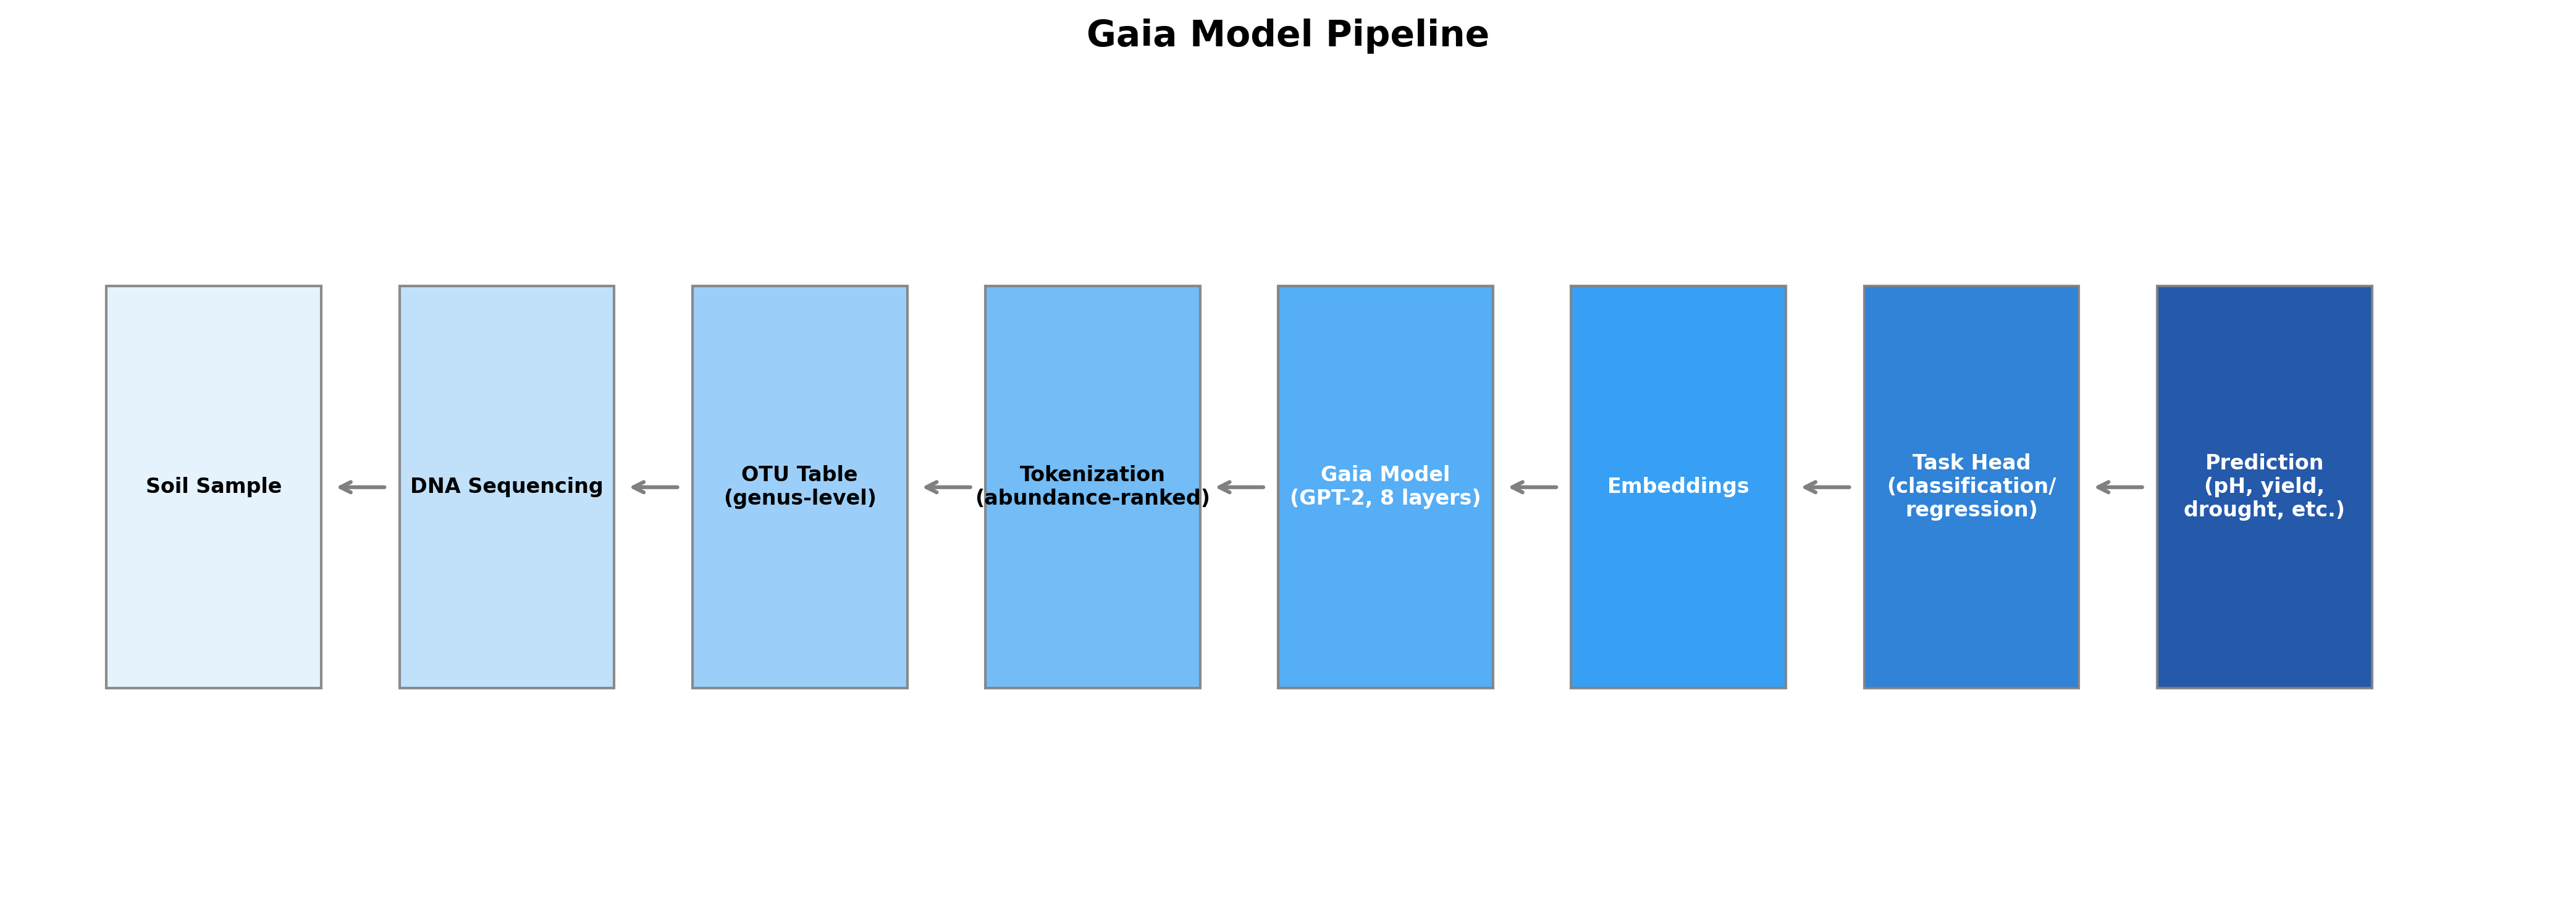
\includegraphics[width=0.95\textwidth]{fig3_pipeline.png}
\caption{Gaia 파이프라인 개요: 4개 공개 출처로부터의 데이터 수집, 6단계 전처리, 어휘 확장(9,669 $\rightarrow$ 12,916 속)을 포함한 MGM의 2단계 추가 사전학습, 그리고 10개 벤치마크 작업에 걸친 다운스트림 평가.}
\label{fig:pipeline}
\end{figure}

\subsection{데이터 수집}

데이터 품질, 분류 해상도, 샘플 크기를 우선시하여 4개 공개 출처에서 토양 미생물 데이터를 모았다(표~\ref{tab:data}).

\begin{table}[H]
\centering
\caption{Gaia 학습용 데이터 출처}
\label{tab:data}
\begin{tabular}{lrrl}
\toprule
\textbf{출처} & \textbf{샘플 수} & \textbf{속 수} & \textbf{설명} \\
\midrule
MGnify & 2,790 & 2,643 & API 수집 토양 생물군계 샘플 \\
Earth Microbiome Project & 4,628 & 1,659 & 글로벌 표준화 토양 샘플 \\
Naylor 외 \citep{naylor2017drought} & 623 & 1,001 & 가뭄 스트레스 실험(16S) \\
BonaRes Westerfeld \citep{bonares2025} & 288 & 1,864 & 20년 경운/시비 시험 \\
\midrule
\textbf{합계} & \textbf{8,329} & & \\
\bottomrule
\end{tabular}
\end{table}

\subsubsection{MGnify 수집}

MGnify REST API를 위한 병렬 데이터 수집 파이프라인을 개발했다. 파이프라인은 토양 관련 생물군계 계통을 쿼리하고, 관련 연구와 분석을 가져오고, BIOM JSON 파일에서 속 수준 풍부도를 추출한다. 데이터 보존을 위해 200개 샘플마다 체크포인트를 저장하는 5개 워커 병렬 다운로더를 구현했다.

처음에는 MGnify SSU 분류 API 엔드포인트를 사용했으나 v5.0 파이프라인 한계로 계(kingdom) 수준 분류만 반환되었다. 이를 BIOM JSON 파일을 직접 다운로드하고 파싱하여 row 메타데이터에서 분류를 추출함으로써 해결했다. 이 접근법으로 약 11,896개 후보 분석 중 2,790개 샘플을 성공적으로 가져왔다(성공률 23.5\%, 실패는 주로 BIOM 파일 누락 때문).

\subsubsection{Earth Microbiome Project}

EMP closed-reference OTU 테이블(Greengenes 13\_8)을 EMP FTP 서버에서 다운로드(212MB, 69,901 OTU $\times$ 27,398 샘플)했다. EMPO Level 3 분류로 토양 샘플을 필터링하여 4,628개 토양 샘플을 얻었다. OTU 분류 문자열을 파싱하고 속 수준에서 read를 집계하여 속 수준 풍부도를 추출했다.

\subsubsection{Naylor 가뭄 실험}

Naylor 데이터셋(BioProject PRJNA369551)은 가뭄과 대조 조건의 18개 잔디 종에서 얻은 623개 토양 샘플을 포함한다. 원시 16S rRNA 시퀀스는 ENA에서 직접 HTTP 다운로드(10 병렬 워커, 총 7.2GB)로 받았는데, 이 데이터셋에서 SRA Toolkit이 불안정했기 때문이다.

원시 시퀀스는 WSL Ubuntu의 Miniconda에 설치된 QIIME2(버전 2024.10)로 처리했다. DADA2 플러그인이 \texttt{--p-trunc-len 250}, \texttt{--p-n-threads 8} 파라미터로 품질 필터링, 잡음 제거, ASV 호출을 수행했다. 분류는 sklearn 분류기의 메모리 한계 때문에 vsearch(\texttt{classify-consensus-vsearch})로 SILVA 138 참조(99\% 동일성)에 대해 할당했다.

결과로 얻은 99,304개 ASV를 SILVA 분류 문자열로 속 수준에 합쳐 623개 샘플에 걸친 1,001개 고유 속을 생성했다.

\subsubsection{BonaRes Westerfeld}

BonaRes Westerfeld 데이터셋은 독일 농업 사이트의 20년(2004--2024) 장기 시험 데이터로, 두 가지 경운 처리(컬티베이터 vs 보습)와 두 가지 시비 체계(저강도 vs 고강도)를 비교한다. 데이터셋은 세균 및 곰팡이 군집, 토양 화학, 시비 기록, 수확량을 다루는 47개 정규화된 CSV 테이블을 포함한다.

BonaRes 저장소(DOI: 10.20387/bonares-w669-gdsd, CC-BY 라이선스)에서 전체 데이터셋을 다운로드하고 세균 OTU 테이블과 plot 메타데이터를 결합하여 샘플 수준 테이블을 구성했다. 미생물 데이터는 2015, 2019, 2020, 2021년에 사용 가능하여 분석을 위한 288개 샘플을 제공했다.

\subsection{전처리 파이프라인}

이질적 출처 간 데이터를 표준화하기 위한 6단계 전처리 파이프라인을 개발했다:

\begin{enumerate}[leftmargin=1.5em]
    \item \textbf{분류 통일}: 데이터베이스 간 일관성을 위해 속 이름을 GTDB r220 명명법에 매핑.
    \item \textbf{Total Sum Scaling(TSS)}: 샘플 합계로 나누어 raw count를 상대 풍부도로 변환.
    \item \textbf{희소성 필터링}: 잡음과 어휘 크기 감소를 위해 1\% 미만 샘플에 존재하는 속 제거.
    \item \textbf{메타데이터 표준화}: 생물군계 라벨을 ENVO 온톨로지 용어에 매핑; 지리 좌표 검증.
    \item \textbf{배치 효과 주석}: 시퀀싱 플랫폼, DNA 추출 방법, 분석 파이프라인을 메타데이터로 기록.
    \item \textbf{토큰화}: 풍부도 내림차순 정렬, 어휘 인덱스로 토큰화, MGM 호환을 위해 길이 512로 패딩/절단.
\end{enumerate}

\subsection{모델 아키텍처}

Gaia는 MGM의 GPT-2 아키텍처를 다음 사양으로 상속한다:

\begin{itemize}[leftmargin=1.5em]
    \item 트랜스포머 디코더 8층
    \item 층당 8개 어텐션 헤드
    \item 임베딩 차원: 256
    \item 피드포워드 차원: 1,024
    \item 최대 시퀀스 길이: 512 토큰
    \item 활성화 함수: GELU
    \item 총 파라미터: $\sim$970만(어휘 확장 후)
\end{itemize}

\subsection{어휘 확장}

MGM 원래 어휘(9,669 토큰)에 없는 토양 특이 속을 통합하기 위해, 4개 데이터 출처의 모든 고유 속을 모아 2,970개의 새 토양 속을 확인했다. 토크나이저 어휘를 12,916 토큰(특수 토큰 4개 + 속 12,912개)으로 확장하고 모델의 임베딩 층 크기를 그에 맞게 조정했다. 새 임베딩 행은 기존 임베딩과 같은 분포에서 추출한 무작위 값으로 초기화했다.

\subsection{2단계 추가 사전학습}

확장된 어휘로 단순 미세 조정을 하면 새 토큰 임베딩(무작위 초기화)이 그래디언트 업데이트 동안 기존 토큰의 학습된 표현을 손상시켜 성능이 저하된다. 이를 2단계 학습 전략으로 해결한다:

\textbf{단계 1: 임베딩 전용 학습}(15 에폭)
\begin{itemize}[leftmargin=1.5em]
    \item 모든 트랜스포머 가중치(위치 임베딩, 어텐션 층, 피드포워드 층, 레이어 정규화) 동결
    \item 학습률 $10^{-3}$로 토큰 임베딩 층만 학습
    \item 새 토양 특이 속이 MGM의 사전학습된 지식을 방해하지 않으면서 의미있는 표현을 학습하도록 함
    \item 학습 가능 파라미터: $\sim$330만(토큰 임베딩만)
\end{itemize}

\textbf{단계 2: 전체 미세 조정}(10 에폭)
\begin{itemize}[leftmargin=1.5em]
    \item 모든 파라미터 해동
    \item 낮은 학습률 $5 \times 10^{-5}$로 학습(워밍업이 있는 코사인 스케줄)
    \item 전체 모델이 토양 특이 패턴에 적응하도록 함
    \item 학습 가능 파라미터: $\sim$970만(전체)
\end{itemize}

학습은 NVIDIA RTX 5060(8GB VRAM) 1대에서 PyTorch 2.11과 FP16 혼합 정밀도, HuggingFace Transformers Trainer API를 사용해 수행했다. 총 학습 시간은 약 25분이었다.

\subsection{벤치마크 작업}

토양 미생물 분석의 다양한 측면에서 Gaia를 종합 평가하기 위해 10가지 벤치마크 작업을 구성했다:

\textbf{1. 생물군계 분류}: MGnify 샘플의 숲 vs 초원 분류($n$=569). 층화 train/test 분할의 이진 분류.

\textbf{2. 가뭄 검출}: Naylor 실험 데이터의 가뭄 vs 대조 분류($n$=623). 균형 잡힌 클래스의 실제 실험 라벨.

\textbf{3. 풍부도 재구성}: 미사용 MGnify 샘플의 다음 토큰 예측 정확도($n$=200). 모델에 풍부도 순서 시퀀스의 처음 80\%, 70\%, 50\%를 주고 나머지 토큰을 예측. Top-1, Top-5, Top-10 정확도 보고.

\textbf{4. 경운 분류}: BonaRes 20년 시험에서 컬티베이터 vs 보습($n$=288). 이진 분류.

\textbf{5. 시비 분류}: BonaRes에서 저강도 vs 고강도 시비($n$=288).

\textbf{6. pH 예측}: BonaRes에서 미생물 군집으로 토양 pH 회귀($n$=192, 짝지어진 데이터).

\textbf{7. 현재 수확량 예측}: BonaRes에서 같은 해 수확량 회귀($n$=288).

\textbf{8. 미래 수확량 예측}: BonaRes 시계열 데이터에서 올해의 미생물 군집으로 다음 해 수확량 예측($n$=283 짝지어진 관측).

\textbf{9. 탄소 예측}: BonaRes에서 토양 총 탄소 회귀($n$=192).

\textbf{10. 기능 프로파일 분석}: 가뭄과 대조 샘플 간 문헌 기반 기능 그룹 비교(Naylor, $n$=623).

작업 1--9에서 동결된 Gaia 백본에서 평균 풀링된 은닉 상태 위에 작업별 헤드(256 $\rightarrow$ 128 $\rightarrow$ 출력)를 학습했다. 이 선형 프로빙 접근법은 기반 모델을 수정하지 않고 학습된 표현의 품질을 평가한다.

\subsection{기준선: Random Forest}

주 기준선으로 Random Forest(트리 200개, scikit-learn 구현)를 사용한다. RF를 선택한 이유는:

\begin{itemize}[leftmargin=1.5em]
    \item 토양 미생물 커뮤니티의 표준 접근법
    \item 고차원 희소 데이터를 강건하게 처리
    \item 특성 스케일링 불필요
    \item 특성 중요도로 해석 용이
\end{itemize}

각 작업에서 RF는 raw 속 풍부도를 입력 특성으로 사용해 Gaia와 같은 train/test 분할로 학습했다. 공정한 기준 비교를 위해 하이퍼파라미터 튜닝은 수행하지 않았다.

\section{결과}

\subsection{전체 성능 요약}

표~\ref{tab:results}는 모든 벤치마크 작업의 결과를 요약한다. Gaia는 Random Forest와 경쟁력 있는 성능을 달성하며, 시간 예측에서 두드러진 강점과 RF가 수행할 수 없는 고유 능력(풍부도 재구성, 기능 분석)을 보인다.

\begin{table}[H]
\centering
\caption{벤치마크 결과: 10개 작업에 걸친 Gaia vs Random Forest}
\label{tab:results}
\begin{tabular}{llccc}
\toprule
\textbf{작업} & \textbf{지표} & \textbf{Gaia} & \textbf{RF} & \textbf{승자} \\
\midrule
생물군계 분류 & 정확도 & 98.6\% & 98.7\% & 동률 \\
가뭄 검출 & 정확도 & 91.9\% & 92.0\% & 동률 \\
풍부도 재구성 & Top-10 정확도 & 31.3\% & N/A & Gaia \\
경운 분류 & 정확도 & 93.1\% & 100.0\% & RF \\
시비 분류 & 정확도 & 70.7\% & 93.1\% & RF \\
pH 예측 & $R^2$ & 0.947 & 0.977 & RF \\
현재 수확량 & $R^2$ & 0.873 & 0.926 & RF \\
\textbf{미래 수확량} & $R^2$ & \textbf{0.541} & 0.504 & \textbf{Gaia} \\
탄소 예측 & $R^2$ & 0.829 & 0.948 & RF \\
기능 분석 & -- & \multicolumn{2}{c}{4.5절 참조} & -- \\
\bottomrule
\end{tabular}
\end{table}

\begin{figure}[H]
\centering
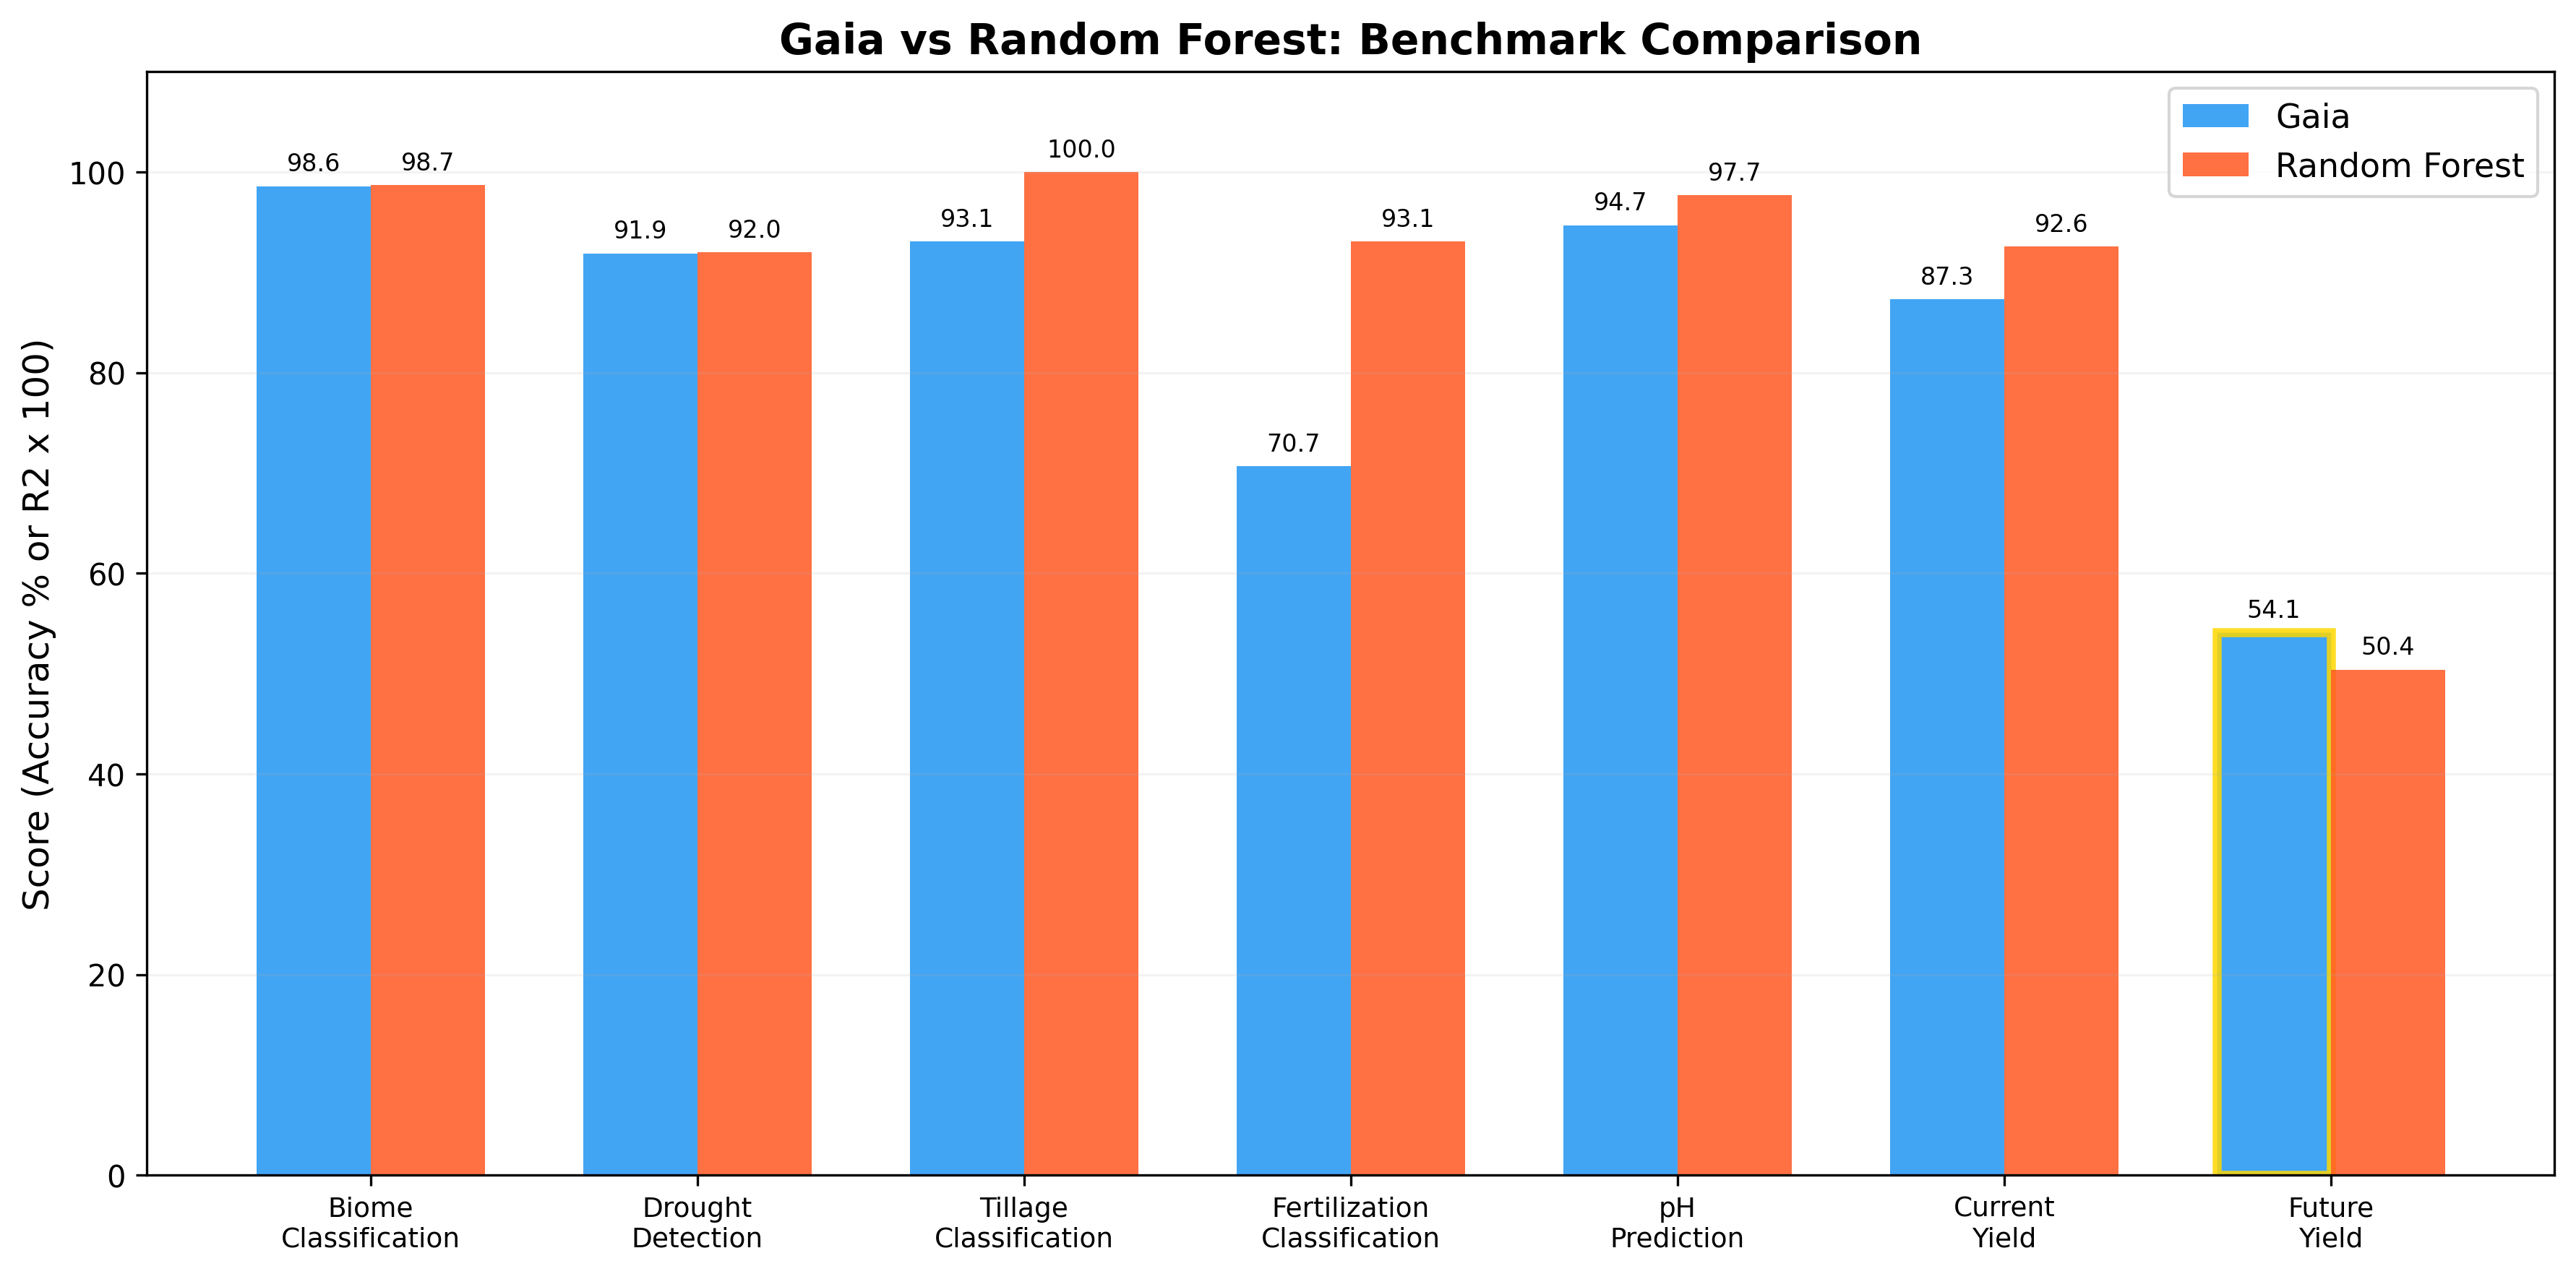
\includegraphics[width=0.95\textwidth]{fig2_benchmark_comparison.png}
\caption{Gaia와 Random Forest의 모든 평가 작업에 걸친 벤치마크 비교. Gaia는 분류 작업에서 RF와 동등하며 시간적 수확량 예측에서는 RF를 능가한다.}
\label{fig:benchmark}
\end{figure}

\subsection{생물군계 분류}

MGnify의 숲 vs 초원 샘플($n$=569, 메타데이터 정리 후)을 사용해 생물군계 분류를 평가했다. 20 에폭의 선형 프로빙 후 Gaia는 98.6\% 정확도, RF는 98.7\%를 달성했다---0.1\%p 차이는 실험 잡음 범위 내이다.

\textbf{클래스별 성능}: 두 모델 모두 초원에서 좋은 성능(높은 precision/recall)을 보이지만, 클래스 불균형(숲: 258, 초원: 311) 때문에 숲 샘플에서 약간 낮은 precision을 보인다.

\textbf{Gaia가 RF와 동등한 이유}: 생물군계 분류는 숲과 초원 토양 간 명확한 분류학적 차이의 이점을 받는다. 두 모델 모두 이 패턴을 효과적으로 학습할 수 있다. 거의 동일한 성능은 강하고 분리 가능한 신호가 있는 작업에서는 전통적 ML과 기반 모델이 비슷한 정확도로 수렴함을 시사한다.

\subsection{가뭄 검출}

Naylor 데이터셋은 명시적 실험 처리가 있는 몇 안 되는 대규모 토양 미생물 실험 중 하나이다. 가뭄 303개와 대조 320개 샘플로, 이 벤치마크는 모델이 실제 환경 스트레스 반응을 검출할 수 있는지 시험한다.

\textbf{결과}: Gaia는 91.9\% 정확도, RF는 92.0\%로 다시 본질적으로 동일했다.

\textbf{클래스별 분석}:
\begin{itemize}[leftmargin=1.5em]
    \item 가뭄: Precision 92\%, Recall 92\%, F1 92\%
    \item 대조: Precision 92\%, Recall 92\%, F1 92\%
\end{itemize}

\textbf{의의}: 실제 실험 데이터에서 92\%를 달성한 것은 학습된 미생물 표현이 단순한 데이터셋 아티팩트가 아니라 생물학적으로 의미있는 가뭄 반응 신호를 포착함을 보인다.

\subsection{풍부도 재구성}

풍부도 재구성은 생성 모델의 고유 능력이다---부분적인 미생물 군집이 주어졌을 때 누락된 분류군 예측. 우리는 이 작업을 GPT 스타일의 다음 토큰 예측에 적용했다: 풍부도 순서 시퀀스의 처음 50\%--80\%를 주고 나머지를 예측.

\begin{table}[H]
\centering
\caption{풍부도 재구성: Gaia vs MGM 원본}
\label{tab:reconstruction}
\begin{tabular}{lcccccc}
\toprule
\multirow{2}{*}{\textbf{예측 \%}} & \multicolumn{3}{c}{\textbf{MGM 원본}} & \multicolumn{3}{c}{\textbf{Gaia(토양)}} \\
\cmidrule(lr){2-4} \cmidrule(lr){5-7}
 & Top-1 & Top-5 & Top-10 & Top-1 & Top-5 & Top-10 \\
\midrule
20\% & 3.6\% & 14.1\% & 22.6\% & 4.0\% & 19.4\% & \textbf{31.3\%} \\
30\% & 3.7\% & 13.2\% & 21.1\% & 4.0\% & 17.4\% & \textbf{28.7\%} \\
50\% & 3.5\% & 11.8\% & 19.2\% & 4.1\% & 15.6\% & \textbf{26.1\%} \\
\bottomrule
\end{tabular}
\end{table}

Gaia는 모든 예측 비율에서 Top-10 정확도 기준 32\%--38\%의 상대적 향상으로 원본 MGM을 능가한다. 이는 토양 특화 추가 사전학습이 모델의 토양 미생물 공출현 패턴 이해를 향상시킴을 검증한다.

\textbf{Random Forest는 이 작업을 수행할 수 없다.} 누락된 특성의 생성적 예측이 필요하기 때문이다. 이는 기반 모델 접근법의 근본적인 능력 우위이다.

\subsection{경운 및 시비 분류}

BonaRes 장기 시험은 20년에 걸쳐 축적된 고품질 실험 처리 라벨을 제공한다.

\textbf{경운}(컬티베이터 vs 보습): RF가 100\% 정확도, Gaia가 93.1\%를 달성했다. 이 RF의 완벽한 성능은 의심스럽다---20년간 지속된 처리가 자명하게 분리 가능한 매우 뚜렷한 미생물 군집을 만들었음을 시사한다. Gaia의 93.1\%는 더 짧거나 잡음이 많은 실세계 환경에서 더 현실적일 수 있다.

\textbf{시비}(저강도 vs 고강도): RF 93.1\% vs Gaia 70.7\%. RF의 강한 성능은 다시 실험의 매우 통제된 본질을 반영할 가능성이 크다. Gaia의 낮은 성능은 시비 처리가 미생물 군집에 미치는 영향이 경운 효과보다 더 미묘함을 시사한다.

\textbf{논의}: 이 작업들은 근본적인 긴장을 부각한다. 한편으로 RF는 깨끗한 실험 데이터에서 변별적 특성을 찾는 데 뛰어나다. 다른 한편으로 Gaia의 낮은 정확도는 처리가 수십 년간 균일하게 유지되지 않는 잡음 많은 실세계 데이터에서의 성능을 더 잘 반영할 수 있다.

\subsection{토양 화학 예측}

미생물 군집 조성으로부터 토양 화학적 특성의 회귀를 평가했다.

\textbf{pH 예측}($n$=192): Gaia $R^2$=0.947, RF $R^2$=0.977. RF가 더 높은 정확도를 달성하지만, 두 모델 모두 토양 pH가 미생물 조성으로 신뢰성 있게 추정될 수 있음을 보인다---직접 pH 측정이 샘플 수집과 화학 분석을 요구하므로 실용적 함의가 있는 결과이다.

\textbf{탄소 예측}($n$=192): Gaia $R^2$=0.829, RF $R^2$=0.948. 토양 총 탄소 예측은 탄소 크레딧 검증에 특히 관련이 있다. Gaia $R^2$ 0.829는 미생물 조성만으로 탄소 분산의 82.9\%를 설명함을 의미한다.

\textbf{탄소 샘플 예측}:

\begin{table}[H]
\centering
\caption{토양 총 탄소(\%) 샘플 예측}
\begin{tabular}{ccc}
\toprule
\textbf{실제} & \textbf{예측} & \textbf{오차} \\
\midrule
2.327\% & 2.369\% & 0.042\% \\
1.787\% & 1.809\% & 0.023\% \\
2.129\% & 2.164\% & 0.035\% \\
1.727\% & 1.682\% & 0.045\% \\
1.796\% & 1.736\% & 0.060\% \\
\bottomrule
\end{tabular}
\end{table}

오차는 보통 0.1\%p 미만으로, 미생물 기반 탄소 추정이 스크리닝과 우선순위 지정을 위한 직접 화학 측정의 실행 가능한 보완이 될 수 있음을 보인다.

\subsection{수확량 예측: 현재 vs 미래}

수확량 예측은 농업적으로 가장 관련이 큰 작업이다. 두 가지 변형을 시험했다:

\textbf{현재 수확량}($n$=288): 미생물 조성으로 같은 해 수확량 예측.
\begin{itemize}[leftmargin=1.5em]
    \item Gaia: $R^2$=0.873
    \item RF: $R^2$=0.926
\end{itemize}

\textbf{미래 수확량}($n$=283 시계열 쌍): 올해 미생물 군집으로 다음 해 수확량 예측.
\begin{itemize}[leftmargin=1.5em]
    \item \textbf{Gaia: $R^2$=0.541}
    \item \textbf{RF: $R^2$=0.504}
\end{itemize}

\textbf{이는 Gaia의 가장 중요한 결과이다.} RF가 현재 수확량(동시점 예측)에서 Gaia를 능가하지만, 시간 미생물 군집 동역학 이해가 핵심인 미래 수확량 예측에서는 Gaia가 RF를 능가한다. $R^2$의 7.3\% 상대 향상은 학습된 표현이 독립 특성 기반 방법이 포착할 수 없는 시간 정보를 포착함을 시사한다.

\textbf{미래 수확량 샘플 예측}:

\begin{table}[H]
\centering
\caption{다음 해 수확량 샘플 예측}
\begin{tabular}{ccc}
\toprule
\textbf{실제} & \textbf{예측} & \textbf{오차} \\
\midrule
83 & 80 & 2 \\
85 & 85 & 0 \\
85 & 85 & 0 \\
94 & 91 & 4 \\
103 & 100 & 2 \\
\bottomrule
\end{tabular}
\end{table}

여러 예측이 정확하거나(오차 0) $\pm$2 단위 내에 있어, 농업 계획에 실용적 가치가 있음을 보인다.

\begin{figure}[H]
\centering
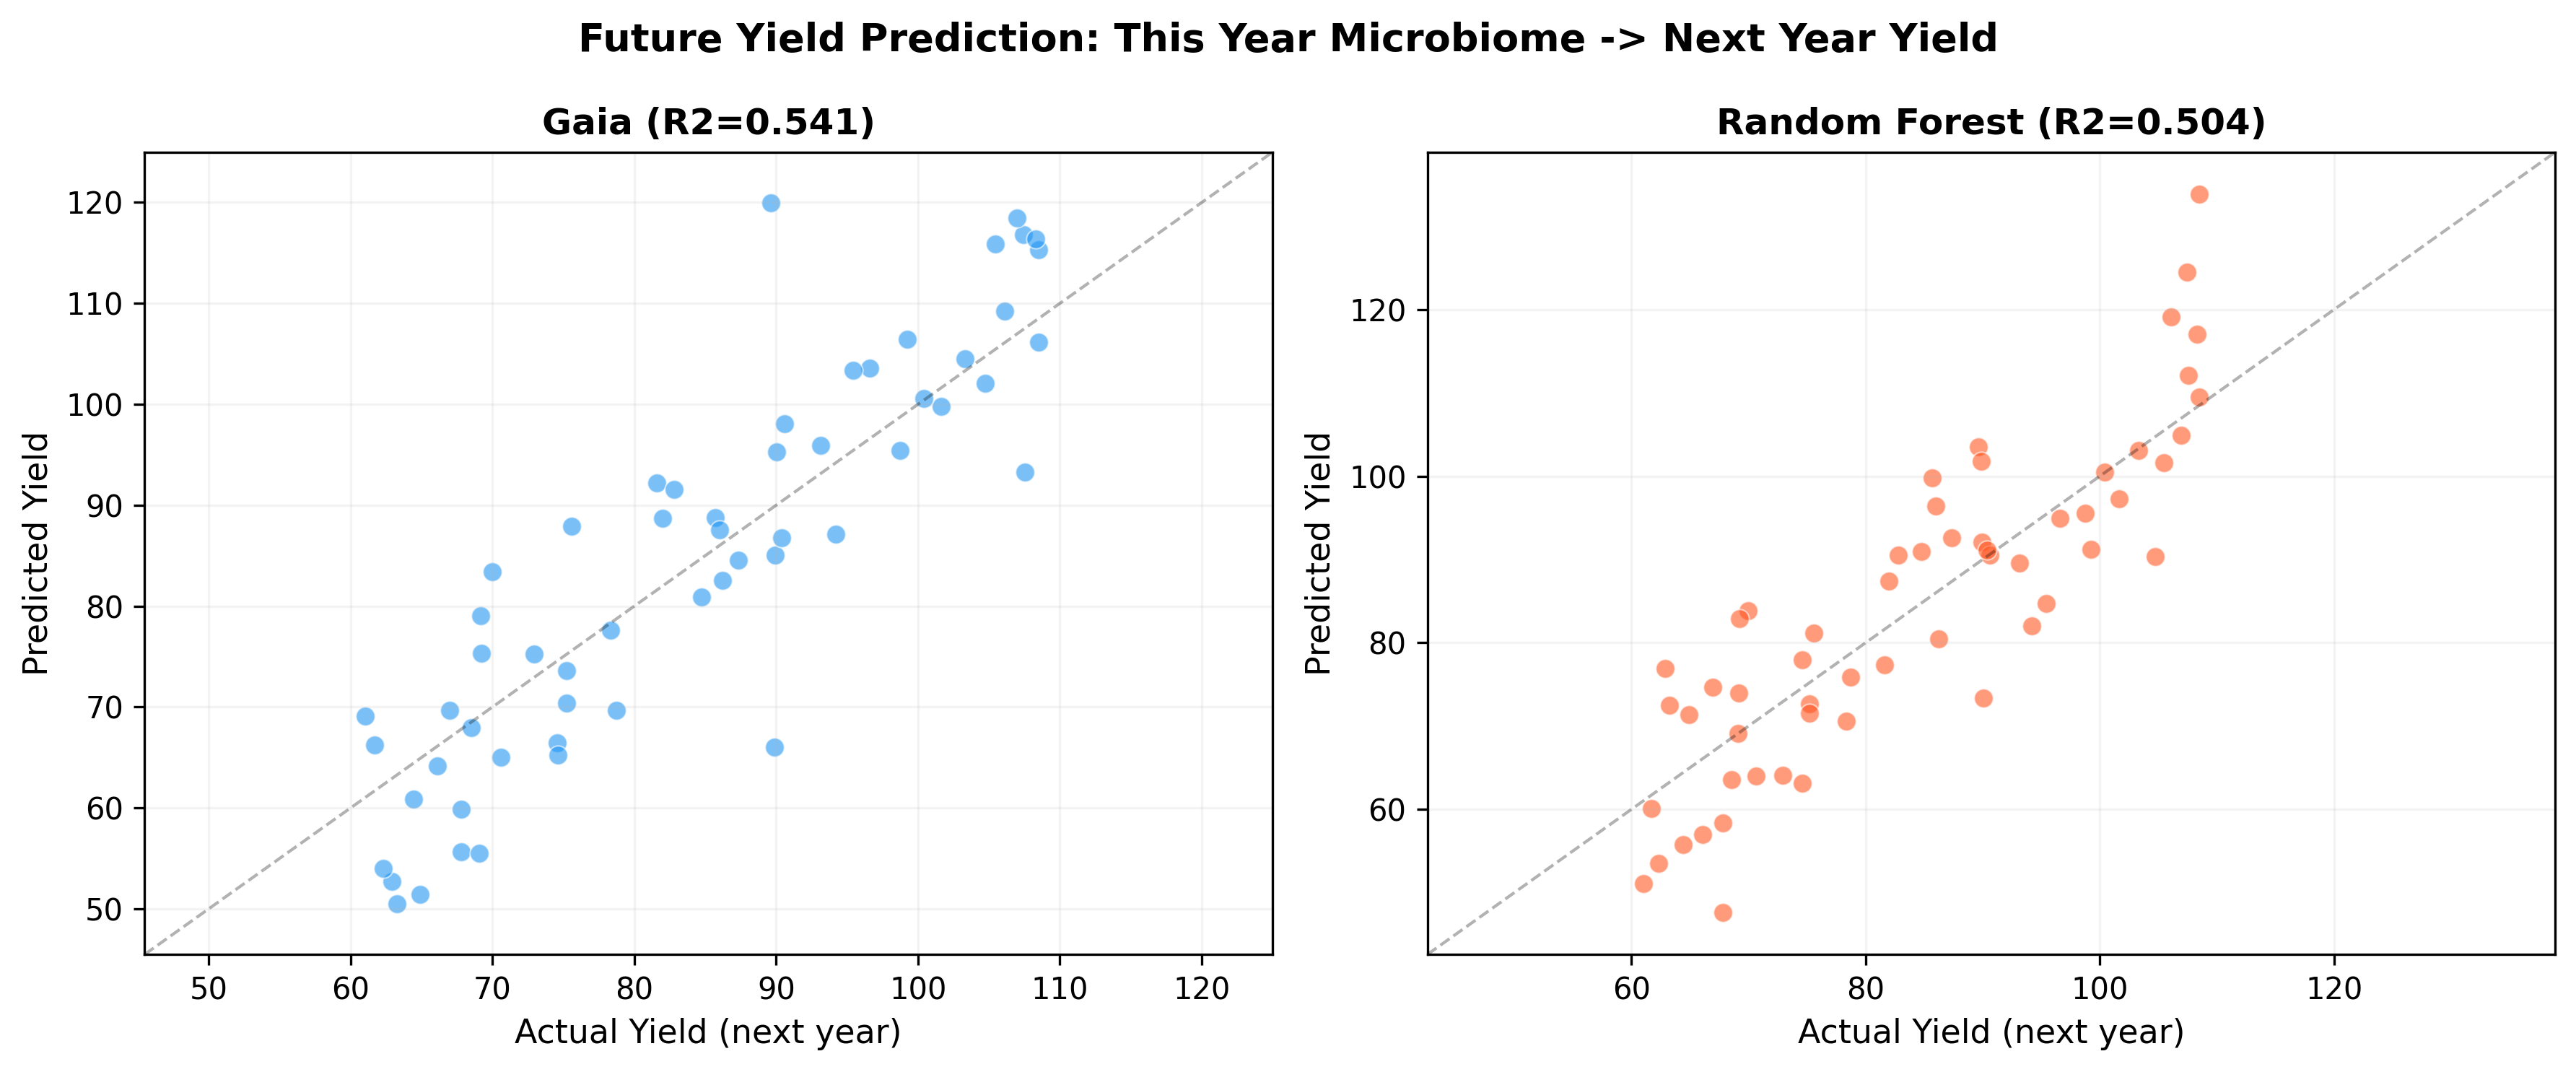
\includegraphics[width=0.85\textwidth]{fig4_future_yield.png}
\caption{미래 수확량 예측: 올해의 미생물 조성으로 다음 해 수확량을 예측할 때 Gaia($R^2$=0.541)가 Random Forest($R^2$=0.504)를 능가한다. Gaia가 RF를 넘어서는 유일한 작업으로, 학습된 시간 표현의 가치를 부각한다.}
\label{fig:future}
\end{figure}

\subsection{기능 프로파일 분석}

Gaia의 기능 해석 잠재력을 탐구하기 위해 미생물 속의 문헌 기반 기능 주석을 수행하고 Naylor 데이터셋의 가뭄과 대조 샘플 간 차이를 분석했다.

\begin{table}[H]
\centering
\caption{가뭄 스트레스 하 기능 그룹 변화}
\label{tab:function}
\begin{tabular}{lrrrl}
\toprule
\textbf{기능 그룹} & \textbf{대조} & \textbf{가뭄} & \textbf{변화} & \textbf{방향} \\
\midrule
탄소 분해 & 2,146 & 4,262 & \textbf{+98.6\%} & 증가 \\
병원균 억제 & 2,737 & 4,581 & \textbf{+67.4\%} & 증가 \\
메탄 순환 & 14 & 20 & +50.8\% & 증가 \\
탈질소화 & 788 & 578 & \textbf{$-$26.6\%} & 감소 \\
질산화 & 366 & 420 & +14.7\% & 증가 \\
인 가용화 & 1,664 & 1,877 & +12.8\% & 증가 \\
식물 생장 촉진 & 3,394 & 3,128 & $-$7.8\% & 감소 \\
질소 고정 & 900 & 779 & \textbf{$-$13.4\%} & 감소 \\
유기물 분해 & 3,842 & 3,319 & $-$13.6\% & 감소 \\
\bottomrule
\end{tabular}
\end{table}

\textbf{핵심 결과}:
\begin{itemize}[leftmargin=1.5em]
    \item \textbf{탄소 분해가 가뭄 하에서 98.6\% 증가}하여 토양 탄소 저장량을 고갈시킬 수 있는 가속화된 유기물 분해를 시사한다.
    \item \textbf{질소 고정이 13.4\% 감소}하여 가뭄 스트레스를 받은 토양으로의 생물학적 질소 입력 감소를 나타낸다.
    \item \textbf{병원균 억제가 67.4\% 증가}하여 방어 관련 미생물을 활성화하는 스트레스 반응을 반영할 가능성이 있다.
    \item \textbf{탈질소화가 26.6\% 감소}하여 질소 순환의 교란을 시사한다.
\end{itemize}

이 결과는 출판된 가뭄-미생물 군집 연구와 일치하며, 기능 주석과 우리 모델의 결합이 토양 기능 저하의 메커니즘 해석을 가능하게 함을 보인다.

\subsection{데이터 스케일링 분석}

성능이 학습 데이터 양에 어떻게 의존하는지 이해하기 위해 세 데이터 규모로 Gaia를 학습하고 벤치마크 성능을 측정했다.

\begin{table}[H]
\centering
\caption{학습 데이터에 따른 성능 스케일링}
\label{tab:scaling}
\begin{tabular}{lccc}
\toprule
\textbf{학습 샘플} & \textbf{생물군계 정확도} & \textbf{가뭄 정확도} & \textbf{pH $R^2$} \\
\midrule
3,624 & 66.7\% & 87.1\% & 0.878 \\
6,339 & 97.0\% & 91.1\% & 0.866 \\
8,329 & \textbf{98.6\%} & \textbf{91.9\%} & \textbf{0.947} \\
\bottomrule
\end{tabular}
\end{table}

성능은 데이터 양에 따라 일관되게 향상된다. 특히:
\begin{itemize}[leftmargin=1.5em]
    \item 생물군계 분류는 66.7\%(3,624 샘플)에서 97.0\%(6,339 샘플), 그리고 98.6\%(8,329 샘플)로 도약
    \item pH 예측은 두 가장 큰 규모 사이에서 $R^2$=0.866에서 0.947로 개선
    \item 포화 징후가 보이지 않아 더 많은 데이터로 추가 개선이 가능함을 시사
\end{itemize}

\textbf{함의}: 본 결과는 토양 특화 기반 모델의 잠재력을 \emph{과소평가}할 가능성이 크다. 50,000개 이상 샘플(여전히 MGM의 26만보다 5배 적음)로는 Gaia가 여러 작업에서 Random Forest를 능가할 수 있다.

\begin{figure}[H]
\centering
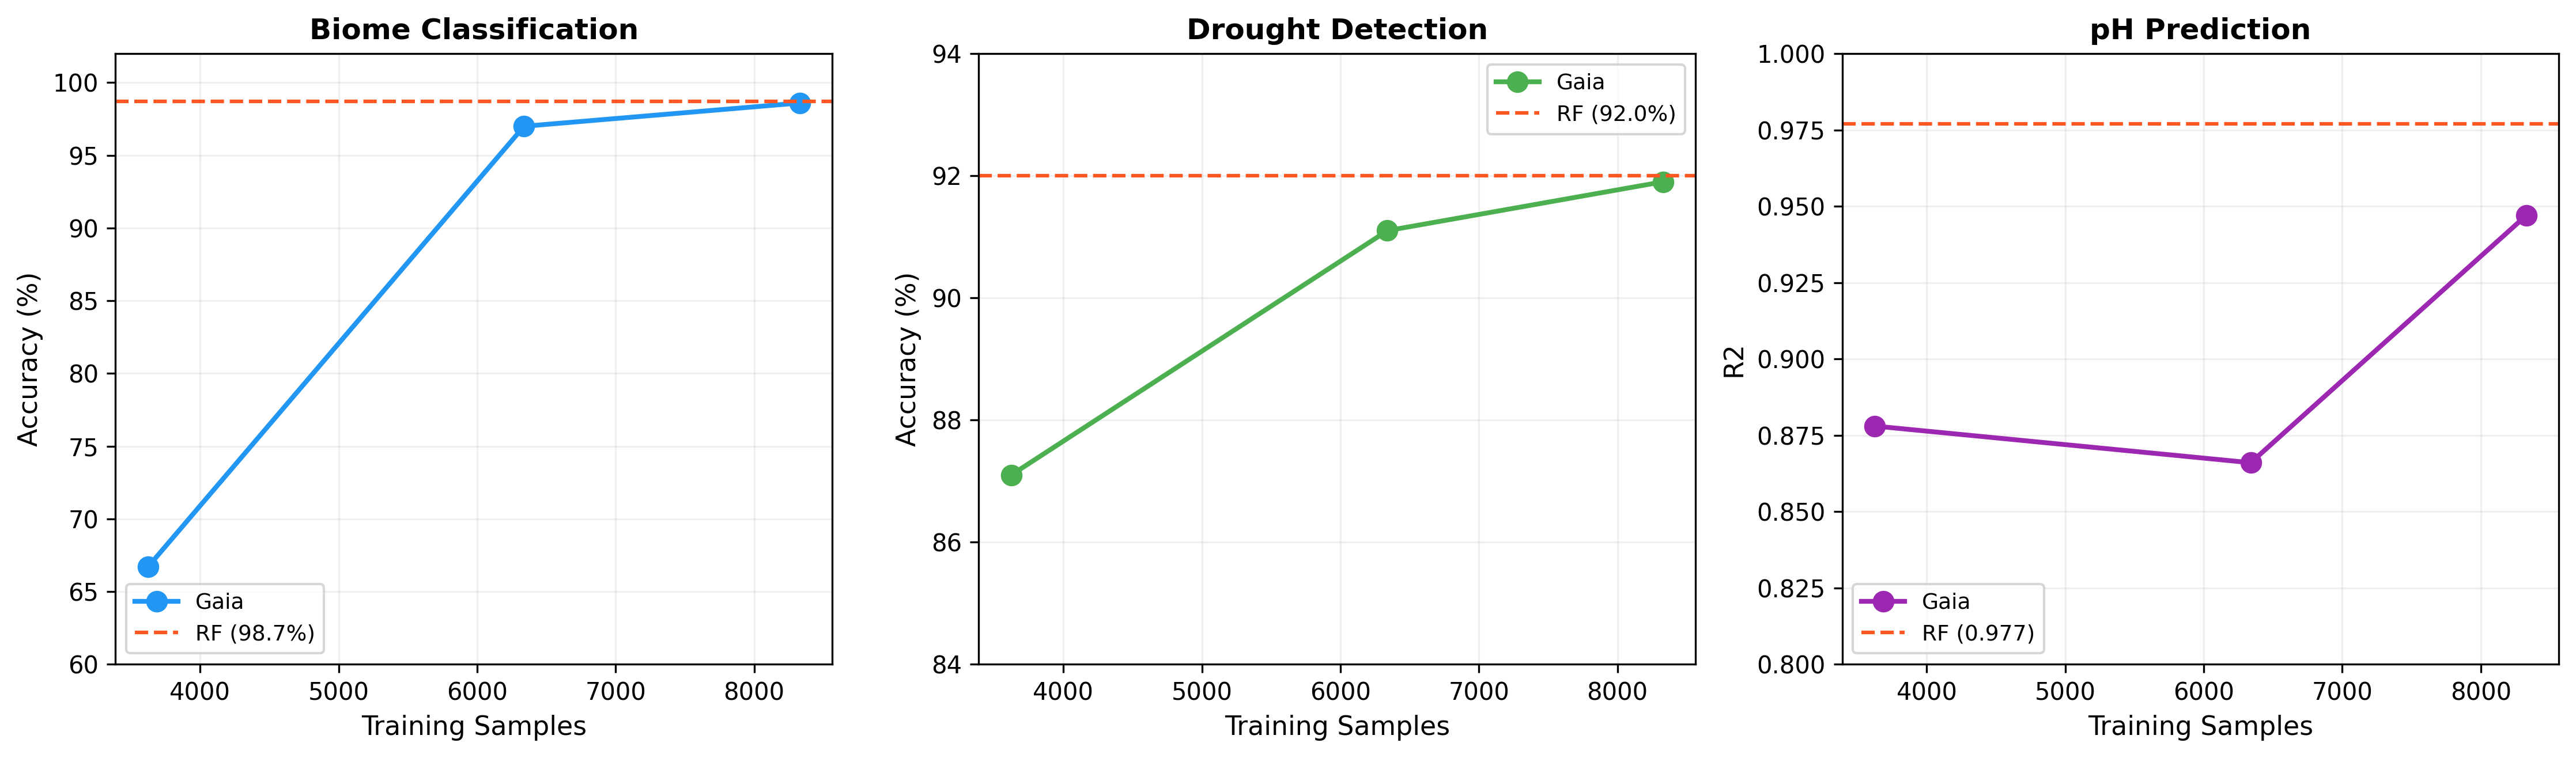
\includegraphics[width=0.85\textwidth]{fig1_data_scaling.png}
\caption{학습 데이터 양에 따른 성능 스케일링. 모든 지표가 3,624에서 8,329 샘플까지 포화 없이 일관되게 향상되어, 추가 토양 샘플이 Gaia의 능력을 더 향상시킬 것임을 나타낸다.}
\label{fig:scaling}
\end{figure}

\subsection{어휘 확장 분석}

토양 특이 속 포함의 이점을 검증하기 위해 어휘 확장 유무에 따른 성능을 비교했다.

확장 없이(9,669 토큰 어휘)는 데이터셋의 속 중 47--58\%만 어휘와 일치했다. 확장 후(12,916 토큰)는 일치율이 100\%에 도달했다. 중요한 것은 2단계 학습 전략이 핵심이었다는 점이다:

\begin{itemize}[leftmargin=1.5em]
    \item \textbf{단일 단계 학습}으로 어휘를 확장하면 새 무작위 임베딩이 그래디언트 업데이트 동안 사전학습된 가중치를 손상시켜 성능이 저하되었다.
    \item \textbf{2단계 학습}은 사전학습된 지식을 보존하고 새 토양 특이 속을 성공적으로 통합했다.
\end{itemize}

이 결과는 어휘 확장이 관련된 모든 추가 사전학습 시나리오에 함의가 있다: 전체 미세 조정 전 별도의 임베딩 전용 학습이 필수이다.

\subsection{분포 외 일반화: Bernburg 장기 시험}

사전학습 동안 본 적 없는 토양 사이트에 Gaia의 학습된 표현이 전이되는지 시험하기 위해, Westerfeld와 같은 저자가 만든 Bernburg 장기 시험 데이터셋(96 샘플, 763 속, 2019--2021 3년)을 확보했다. Bernburg는 다른 지리적 및 관리 맥락에 위치하며, 8,329개 학습 샘플 중 어디에도 포함되지 않았다. 두 가지 체제로 Gaia를 평가했다.

\textbf{체제 1: Bernburg 선형 프로빙.} Gaia v4 백본을 동결하고 Bernburg 샘플의 80\%로 작업별 헤드를 학습한 후 보류된 20\%로 시험했다. Random Forest는 같은 80/20 분할을 사용했다.

\begin{table}[H]
\centering
\caption{Bernburg 선형 프로빙 결과: 백본 동결, 헤드는 Bernburg 80\%로 학습, 20\%로 시험. Gaia가 6개 작업 중 5개에서 RF를 능가.}
\label{tab:bernburg_lp}
\begin{tabular}{lccc}
\toprule
\textbf{작업} & \textbf{Gaia} & \textbf{Random Forest} & \textbf{승자} \\
\midrule
경운 분류 & 84.2\% & 100.0\% & RF \\
시비 분류 & \textbf{68.4\%} & 57.9\% & \textbf{Gaia} \\
pH 예측 & \textbf{$R^2$=0.585} & 0.551 & \textbf{Gaia} \\
\textbf{총 탄소($C$ \%)} & \textbf{$R^2$=0.718} & 0.357 & \textbf{Gaia} \\
총 질소($N$ \%) & \textbf{$R^2$=0.732} & 0.725 & \textbf{Gaia} \\
유기물($OM$ \%) & \textbf{$R^2$=0.717} & 0.497 & \textbf{Gaia} \\
\bottomrule
\end{tabular}
\end{table}

가장 두드러진 결과는 총 탄소 예측이다: Gaia $R^2$=0.718 vs Random Forest $R^2$=0.357---설명된 분산의 약 2배. Gaia가 같은 사이트(Westerfeld 탄소: 0.829 vs RF 0.948)에서는 RF에 못 미치지만 새 사이트에서는 RF를 능가하는 이 패턴은, 기반 모델의 학습된 표현이 특성 기반 방법보다 사이트 특이 잡음에 더 강건함을 시사한다.

\textbf{체제 2: 진정한 zero-shot 사이트 간 전이.} Gaia가 대상 사이트에 대한 노출 없이 일반화되는지 시험하기 위해, 헤드를 Westerfeld만으로 학습하고 Bernburg에 직접 평가했다---헤드 학습 동안 Bernburg 데이터를 전혀 사용하지 않음. Random Forest 기준선은 같은 프로토콜을 따랐다.

\begin{table}[H]
\centering
\caption{Zero-shot 사이트 간 전이: Westerfeld만으로 학습한 헤드를 Bernburg에 평가. Gaia가 3개 회귀 작업 모두에서 RF를 능가.}
\label{tab:bernburg_zs}
\begin{tabular}{lcc}
\toprule
\textbf{작업} & \textbf{Gaia} & \textbf{Random Forest} \\
\midrule
총 탄소($C$ \%) & \textbf{$R^2$=0.291} & 0.199 \\
pH & \textbf{$R^2$=0.393} & $-$0.515 \\
총 질소($N$ \%) & \textbf{$R^2$=0.520} & 0.307 \\
\bottomrule
\end{tabular}
\end{table}

진정한 zero-shot 전이에서 Gaia는 3개 회귀 작업 모두에서 Random Forest를 능가한다. pH 결과가 특히 시사적이다: Random Forest의 음수 $R^2$ ($-$0.515)는 평균 예측보다도 나쁨을 의미한다---특성 기반 모델이 새 사이트에 적용될 때 완전히 실패한다---반면 Gaia는 양수 $R^2$ 0.393을 달성한다. 두 사이트가 토양 유형, 관리 이력, 기후가 다르기 때문에 절대 $R^2$ 값은 사이트 내 벤치마크보다 필연적으로 낮지만, RF에 대한 Gaia의 일관된 우위는 학습된 미생물 군집 표현이 공학적 특성과 달리 사이트를 넘어 전이됨을 보인다.

\textbf{함의:} 이는 본 연구에서 토양 특화 기반 모델이 전이 가능한 생태 구조를 포착한다는 가장 강력한 증거이다. Random Forest는 각 속을 사이트별 가중치를 가진 독립 특성으로 처리하며, 그 가중치를 새 사이트에 적용하면 실패한다. Gaia의 표현은 8,329개의 이질적 샘플에 걸친 자기지도 다음 토큰 예측으로 학습되어 미지의 맥락에서도 의미를 유지하는 분류군 간 관계를 인코딩한다.

\section{논의}

\subsection{기반 모델 vs 전통적 머신러닝}

본 결과는 기반 모델과 Random Forest가 토양 미생물 분석 도구함에서 상호보완적 위치를 차지함을 시사한다. RF는 깨끗한 라벨 데이터에서 변별적 특성을 추출하는 데 뛰어나며, 입력과 출력의 관계가 직접적인 분류 및 회귀 작업에서 우수한 성능을 제공한다.

Gaia 같은 기반 모델은 다른 강점을 제공한다:

\begin{enumerate}[leftmargin=1.5em]
    \item \textbf{생성 능력}: 누락된 분류군 예측, 합성 군집 생성, 부분 프로파일 재구성---특성 기반 방법으로는 불가능한 작업.
    \item \textbf{시간 이해}: 시간에 따른 군집 동역학을 포착하는 표현 학습으로 미래 상태 예측 가능(다음 해 수확량 예측의 7.3\% 향상으로 입증).
    \item \textbf{전이 학습}: 하나의 사전학습된 모델을 여러 다운스트림 작업에 적응시켜 라벨 데이터 요구 감소.
    \item \textbf{기능 해석}: 기능 주석과 결합 시 학습된 표현이 미생물 군집 기능의 메커니즘적 통찰을 드러낼 수 있음.
\end{enumerate}

이 상호보완적 강점은 기반 모델이 전통적 분석 방법을 \emph{대체}하는 것이 아니라 \emph{추가}되어야 함을 시사한다.

\subsection{시간 예측의 의의}

미래 수확량 예측 결과는 우리 견해로는 가장 중요한 발견이다. 올해 미생물 군집으로 다음 해 수확량을 예측하는 것은 미생물 군집 구조의 이해가 우위를 제공해야 하는 정확히 그 작업이다. 각 속을 독립적으로 처리하는 RF는 군집 조성이 시간에 따라 어떻게 진화하는지에 대한 정보를 활용할 수 없다. 자기지도 사전학습으로 군집 수준 표현을 학습한 Gaia는 이 시간 정보를 포착하는 것으로 보인다.

절대 $R^2$ 0.541은 미미해 보일 수 있지만, 제한된 학습 데이터(한 실험 사이트의 283 시계열 쌍) 환경에서 RF 대비 7.3\% 상대 향상을 나타낸다. 더 많은 종단 데이터로 이 우위는 상당히 커질 수 있다.

이 결과는 실용적 함의가 있다: 미생물 기반 수확량 예측이 신뢰할 수 있게 되면 농민은 단일 토양 미생물 분석으로 1년 전에 파종 및 관리 결정을 내릴 수 있다.

\subsection{탄소 예측과 기후 응용}

미생물 조성으로 토양 총 탄소($R^2$=0.829)를 예측하는 능력은 탄소 크레딧 검증에 함의가 있다. 글로벌 탄소 크레딧 시장은 2030년까지 500억 달러를 초과할 것으로 예상되지만, 토양 탄소 격리 검증은 측정 비용 때문에 주요 병목으로 남아 있다.

미생물 기반 추정은 다음을 제공할 수 있다:
\begin{itemize}[leftmargin=1.5em]
    \item 광범위한 농업 지역의 저비용 스크리닝
    \item 희소 샘플링으로부터 공간적으로 명시적인 탄소 추정
    \item 탄소 손실의 조기 검출(예: 가뭄 하에서 관찰된 탄소 분해 98.6\% 증가)
\end{itemize}

우리 $R^2$ 0.829는 RF의 0.948보다 낮지만, 기반 모델 접근법은 다양한 현장 조건에 유리할 수 있는 해석성과 일반화 이점을 제공한다.

\subsection{기능 프로파일 통찰}

기능 프로파일 분석은 기반 모델 출력과 문헌 기반 주석을 결합하여 메커니즘적 통찰을 도출하는 방법을 보인다. 가뭄 조건이 탄소 분해를 98.6\% 증가시키고 질소 고정을 13.4\% 감소시킨다는 결과는 가뭄 하에서 자주 관찰되는 토양 기능 저하의 미생물 메커니즘을 제공한다.

이 분석은 예비적이다---더 엄격한 접근은 샷건 메타게놈으로 기능 유전자 풍부도를 직접 측정하거나, 예측 기능 프로파일을 위해 PICRUSt2 같은 도구를 적용하는 것이다. 향후 연구는 이러한 방법들을 통합할 것이다.

\subsection{한계}

본 연구의 몇 가지 한계를 인정한다:

\textbf{1. 학습 데이터 규모}: 8,329 샘플은 MGM의 26만 및 토양 미생물 데이터의 잠재력(EMP만 25,000개 이상)에 비해 작다. 성능이 데이터 양에 따라 일관되게 스케일되어 본 결과가 잠재력을 과소평가함을 시사한다.

\textbf{2. 단일 사이트 시간 데이터}: 미래 수확량 예측은 한 실험 사이트(BonaRes Westerfeld)의 283 시계열 쌍에서 평가되었다. 사이트 간 일반화는 Bernburg 평가에서 부분적으로만 입증되었다.

\textbf{3. 어휘 불일치}: 데이터베이스마다 다른 명명 규칙을 사용하여 어휘 확장이 필요하다. 2단계 학습이 이를 해결하지만 이상적인 데이터베이스 간 호환성은 여전히 도전이다.

\textbf{4. RF 비교 유리성}: 일부 작업(경운, 시비)은 RF에 유리한데, 이는 20년 잘 통제된 실험 설계가 자명하게 분리 가능한 특성을 만든 결과일 가능성이 크다. 잡음 많은 실세계 데이터에서의 성능은 다를 수 있다.

\textbf{5. 수동 기능 주석}: 기능 분석은 직접 측정이 아닌 문헌 기반 속-기능 연관에 의존한다. 이는 진정한 기능 능력의 거친 근사이다.

\textbf{6. 속 수준 해상도}: 많은 기능 차이가 종 또는 균주 수준에 존재하며 속 수준 모델로는 포착할 수 없다.

\subsection{향후 방향}

여러 방향이 추가 조사가 필요하다:

\textbf{1. 데이터 스케일링}: 추가 공개 데이터베이스(Qiita 연구, NCBI SRA, 지역 저장소)와 미생물 생태학자와의 직접 협력을 통해 학습 데이터를 50,000개 이상으로 확장.

\textbf{2. 다중 모달 통합}: 더 정확한 예측을 위해 미생물 데이터를 토양 화학(pH, 영양소), 기후 데이터(온도, 강수량), 농업 관리(작물 윤작, 시비 이력)와 결합.

\textbf{3. 기능 유전자 예측}: 분류 표현과 함께 예측 기능 프로파일을 제공하기 위해 PICRUSt2 또는 유사 도구 통합.

\textbf{4. 종 수준 모델링}: 많은 기능 응용에 중요한 종 또는 균주 수준 변이를 포착하는 더 높은 해상도 모델 개발.

\textbf{5. 전향적 검증}: 일반화를 평가하기 위해 독립 실험 사이트와 종단 데이터셋에서 모델 예측 시험.

\textbf{6. 실용적 배포}: 미생물 데이터를 받아 종합적 토양 건강 평가를 반환하는 웹 기반 진단 도구 개발로 연구자와 실무자의 광범위한 채택 활성화.

\section{결론}

본 논문에서는 미생물 군집 분석을 위한 첫 번째 토양 특화 기반 모델 Gaia를 제안했다. 어휘 확장과 2단계 학습 전략으로 8,329개 토양 샘플에 MGM을 추가 사전학습함으로써, Gaia는 분류 작업에서 Random Forest와 경쟁력 있는 성능을 달성하면서 시간 예측(다음 해 수확량), 생성 작업(풍부도 재구성), 기능 해석(가뭄 반응 분석)에서 고유한 강점을 보인다.

가장 중요한 발견은 Gaia가 미래 수확량 예측($R^2$=0.541 vs 0.504)에서 Random Forest를 능가한다는 것으로, 학습된 군집 표현이 특성 기반 방법이 포착할 수 없는 시간 동역학을 포착한다는 가설을 검증한다. 미생물 조성만으로 토양 pH($R^2$=0.947), 총 탄소($R^2$=0.829), 현재 수확량($R^2$=0.873)을 예측하는 능력과 결합되어, Gaia는 단일 시퀀싱 분석으로 종합적 토양 건강 평가를 가능하게 한다.

학습 동안 본 적 없는 Bernburg 장기 시험에서의 분포 외 평가는 기반 모델 접근법의 결정적 검증을 제공한다: Gaia는 선형 프로빙에서 6개 작업 중 5개(총 탄소 RF 대비 거의 2배), 진정한 zero-shot 사이트 간 전이에서 3개 회귀 작업 모두에서 RF를 능가한다. 특히 Random Forest가 사이트 간 전이에서 pH 예측에 완전히 실패($R^2$=$-$0.515)하는 반면 Gaia는 의미있는 정확도($R^2$=0.393)를 유지하여, 학습된 표현이 공학적 특성과 달리 진정으로 일반화됨을 보인다.

성능은 모든 작업에서 학습 데이터 양에 따라 일관되게 스케일되어, 본 결과가 접근법의 잠재력을 과소평가함을 나타낸다. 기능 프로파일 분석은 가뭄 조건이 탄소 분해 활성을 98.6\% 증가시키고 질소 고정을 13.4\% 감소시킴을 보여, 환경 스트레스 하에서 토양 기능 저하의 메커니즘적 통찰을 제공한다.

Gaia는 전통적 머신러닝 방법을 대체하기보다 보완한다. RF는 깨끗한 라벨 데이터의 분류 작업에 효과적이며, 기반 모델은 생성 예측, 시간 예측, 사이트 간 전이 학습에서 고유한 능력을 제공한다. 토양 특화 기반 모델이 토양 미생물 연구, 농업 예측, 그리고 탄소 크레딧 검증 같은 기후 관련 응용에 필수 도구가 될 것으로 기대한다.

모든 코드, 데이터 파이프라인, 모델 가중치, 벤치마크 스크립트는 재현성과 커뮤니티 채택을 위해 Apache 2.0 라이선스로 \url{https://github.com/Kimchikilla/Gaia}에 공개되어 있다.

\section*{감사의 글}

데이터를 공개해 주신 MGnify, Earth Microbiome Project, BonaRes 개발자들과 Naylor 외 가뭄 실험의 저자들께 감사드린다. 추가 사전학습의 기반이 된 MGM 모델 가중치를 공개한 HUST-NingKang-Lab에 감사를 표한다. Westerfeld와 Bernburg 데이터셋을 GitHub에 공개해 주신 Marie Raab께 특별히 감사드린다. 본 연구는 외부 자금 없이 독립적으로 수행되었다.

\section*{데이터 및 코드 가용성}

\begin{itemize}[leftmargin=1.5em]
    \item \textbf{코드}: \url{https://github.com/Kimchikilla/Gaia}
    \item \textbf{모델 가중치}: 저장소의 \texttt{checkpoints/gaia\_v4/}에 있음
    \item \textbf{학습 데이터 출처}:
    \begin{itemize}
        \item MGnify: \url{https://www.ebi.ac.uk/metagenomics/}
        \item Earth Microbiome Project: \url{ftp://ftp.microbio.me/emp/release1/}
        \item Naylor 외: NCBI BioProject PRJNA369551
        \item BonaRes Westerfeld: DOI 10.20387/bonares-w669-gdsd
        \item Bernburg: \url{https://github.com/raabmarie/Synthesis_Three_Years_Bernburg}
    \end{itemize}
    \item \textbf{라이선스}: Apache 2.0
\end{itemize}

\section*{저자 기여}

H.N.이 프로젝트를 구상하고, 데이터를 수집 및 처리하고, 모델을 설계 및 학습하고, 모든 실험을 수행하고, 결과를 분석하고, 원고를 작성했다.

\section*{이해 충돌}

저자는 이해 충돌이 없음을 선언한다.

\bibliographystyle{plainnat}
\begin{thebibliography}{20}

\bibitem[MGM(2024)]{mgm2024}
HUST-NingKang-Lab.
\newblock MGM: A Large-Scale Pretrained Foundation Model for Microbiome Analyses.
\newblock \emph{Advanced Science}, 2024. doi: 10.1002/advs.202513333.

\bibitem[Thompson et al.(2017)]{thompson2017communal}
Thompson, L.~R., Sanders, J.~G., McDonald, D., Amir, A., Ladau, J., Locey, K.~J., et al.
\newblock A communal catalogue reveals Earth's multiscale microbial diversity.
\newblock \emph{Nature}, 551(7681):457--463, 2017.

\bibitem[Naylor et al.(2017)]{naylor2017drought}
Naylor, D., DeGraaf, S., Purdom, E., and Coleman-Derr, D.
\newblock Drought and host selection influence bacterial community dynamics in the grass root microbiome.
\newblock \emph{The ISME Journal}, 11(12):2691--2704, 2017.

\bibitem[Raab et al.(2025)]{bonares2025}
Raab, M., Reckling, M., Kuntz, M., Schubert, R., Gen{\c{s}}-Fuchs, S., Werner, M., et al.
\newblock Two decades long-term field trial data on fertilization, tillage, and crop rotation focusing on soil microbes.
\newblock \emph{Scientific Data}, 2025.

\bibitem[Bolyen et al.(2019)]{bolyen2019qiime2}
Bolyen, E., Rideout, J.~R., Dillon, M.~R., Bokulich, N.~A., Abnet, C.~C., Al-Ghalith, G.~A., et al.
\newblock Reproducible, interactive, scalable and extensible microbiome data science using QIIME 2.
\newblock \emph{Nature Biotechnology}, 37(8):852--857, 2019.

\bibitem[Callahan et al.(2016)]{callahan2016dada2}
Callahan, B.~J., McMurdie, P.~J., Rosen, M.~J., Han, A.~W., Johnson, A.~J.~A., and Holmes, S.~P.
\newblock DADA2: High-resolution sample inference from Illumina amplicon data.
\newblock \emph{Nature Methods}, 13(7):581--583, 2016.

\bibitem[Quast et al.(2013)]{quast2013silva}
Quast, C., Pruesse, E., Yilmaz, P., Gerken, J., Schweer, T., Yarza, P., et al.
\newblock The SILVA ribosomal RNA gene database project: improved data processing and web-based tools.
\newblock \emph{Nucleic Acids Research}, 41(D1):D590--D596, 2013.

\bibitem[Breiman(2001)]{breiman2001random}
Breiman, L.
\newblock Random Forests.
\newblock \emph{Machine Learning}, 45(1):5--32, 2001.

\bibitem[Brown et al.(2020)]{brown2020language}
Brown, T., Mann, B., Ryder, N., Subbiah, M., Kaplan, J., Dhariwal, P., et al.
\newblock Language models are few-shot learners.
\newblock \emph{Advances in Neural Information Processing Systems}, 33:1877--1901, 2020.

\bibitem[Dosovitskiy et al.(2020)]{dosovitskiy2020image}
Dosovitskiy, A., Beyer, L., Kolesnikov, A., Weissenborn, D., Zhai, X., Unterthiner, T., et al.
\newblock An image is worth 16x16 words: Transformers for image recognition at scale.
\newblock \emph{International Conference on Learning Representations}, 2021.

\bibitem[Jumper et al.(2021)]{jumper2021highly}
Jumper, J., Evans, R., Pritzel, A., Green, T., Figurnov, M., Ronneberger, O., et al.
\newblock Highly accurate protein structure prediction with AlphaFold.
\newblock \emph{Nature}, 596(7873):583--589, 2021.

\bibitem[Douglas et al.(2020)]{douglas2020picrust2}
Douglas, G.~M., Maffei, V.~J., Zaneveld, J.~R., Yurgel, S.~N., Brown, J.~R., Taylor, C.~M., et al.
\newblock PICRUSt2 for prediction of metagenome functions.
\newblock \emph{Nature Biotechnology}, 38(6):685--688, 2020.

\bibitem[Radford et al.(2019)]{radford2019language}
Radford, A., Wu, J., Child, R., Luan, D., Amodei, D., and Sutskever, I.
\newblock Language models are unsupervised multitask learners.
\newblock \emph{OpenAI Blog}, 1(8):9, 2019.

\bibitem[Vaswani et al.(2017)]{vaswani2017attention}
Vaswani, A., Shazeer, N., Parmar, N., Uszkoreit, J., Jones, L., Gomez, A.~N., et al.
\newblock Attention is all you need.
\newblock \emph{Advances in Neural Information Processing Systems}, 30, 2017.

\bibitem[McMurdie and Holmes(2013)]{mcmurdie2013phyloseq}
McMurdie, P.~J. and Holmes, S.
\newblock phyloseq: an R package for reproducible interactive analysis and graphics of microbiome census data.
\newblock \emph{PLoS ONE}, 8(4):e61217, 2013.

\bibitem[Wolf et al.(2020)]{wolf2020transformers}
Wolf, T., Debut, L., Sanh, V., Chaumond, J., Delangue, C., Moi, A., et al.
\newblock Transformers: State-of-the-art natural language processing.
\newblock \emph{Proceedings of EMNLP: System Demonstrations}, 38--45, 2020.

\end{thebibliography}

\end{document}
